\documentclass[a4paper,twoside]{report}

%%%%%%%%%%%%%%%%%%%%%%%%%%%%%%%%%%
\newcommand{\rtbyear}{2019}
%%%%%%%%%%%%%%%%%%%%%%%%%%%%%%%%%%


\usepackage{times}
\usepackage{graphicx}
\usepackage{wrapfig}
\usepackage{pdfpages}

\usepackage{fancyhdr}
\usepackage[overlay]{textpos}
\usepackage{mathptmx}
\usepackage{anyfontsize}
\usepackage{longtable}
\usepackage{amsfonts}  % mathbb font

\usepackage{t1enc}
\usepackage{booktabs,longtable}

% hyperlinks
\usepackage{hyperref}
\hypersetup{
  colorlinks=true,
  linkcolor=black
  }
  
\usepackage{color}
\usepackage{sectsty}
\usepackage{textcomp}     % access \textquotesingle
\allsectionsfont{\sffamily}
\makeatletter
\newcommand\funcsection{%
\@startsection{section}{1}{\z@}%
  {-3.5ex \@plus -1ex \@minus -.2ex}%
  {2.3ex \@plus.2ex}%
  {\color{red}\sffamily\huge\bfseries}}
\makeatother

%% layout
\def\topfraction{.9}
\def\bottomfraction{.9}
\def\textfraction{.1}
\def\floatpagefraction{.9}

% paragraphs
\usepackage{parskip}
\setlength{\parindent}{0mm}

% space around longtables
\setlength{\LTpre}{6pt}
\setlength{\LTpost}{0pt}

% reduce space around headings
\usepackage[compact]{titlesec}
\titlespacing{\section}{0pt}{*0}{*0}
\titlespacing{\subsection}{0pt}{*0}{*0}
\titlespacing{\subsubsection}{0pt}{*0}{*0}

\renewcommand{\today}{\number\day \space%
\ifcase \month \or January\or February\or March\or April\or May%
\or June\or July\or August\or September\or October\or November\or December\fi, \number \year}
\IfFileExists{../../RELEASE}{\def\release{\input{../../RELEASE}}
\def\reldate{\today}}{\input{release.tex}}



%\usepackage{multind}
\usepackage{multicol}

% printindex stuff

\makeatletter
\def\printindex#1#2{\subsection*{#2}
  \@input{#1.ind}}
  
\def\theindex{\parindent\z@
\parskip\z@ plus .3pt\relax\let\item\@idxitem}
\def\@idxitem{\par\hangindent 40pt}
\def\subitem{\par\hangindent 40pt \hspace*{20pt}}
\def\subsubitem{\par\hangindent 40pt \hspace*{30pt}}
\def\endtheindex{}
\def\indexspace{\par \vskip 10pt plus 5pt minus 3pt\relax}
\makeatother

\usepackage{fancyvrb}
\fvset{formatcom=\color{blue},fontseries=c,fontfamily=courier,xleftmargin=4mm,commentchar=!}
\DefineVerbatimEnvironment{Code}{Verbatim}{formatcom=\color{blue},fontseries=c,fontfamily=courier,fontsize=\footnotesize,xleftmargin=4mm,commentchar=!}
\pagestyle{empty}

\def\Mlab{MATLAB}

\begin{document}
\typeout{**Starting}
\setlength{\TPHorizModule}{1cm}
\setlength{\TPVertModule}{1cm}

%%%%%%%%%%%%%%%%% TITLE PAGE
\begin{textblock}{19}(-3.5,-4.5)
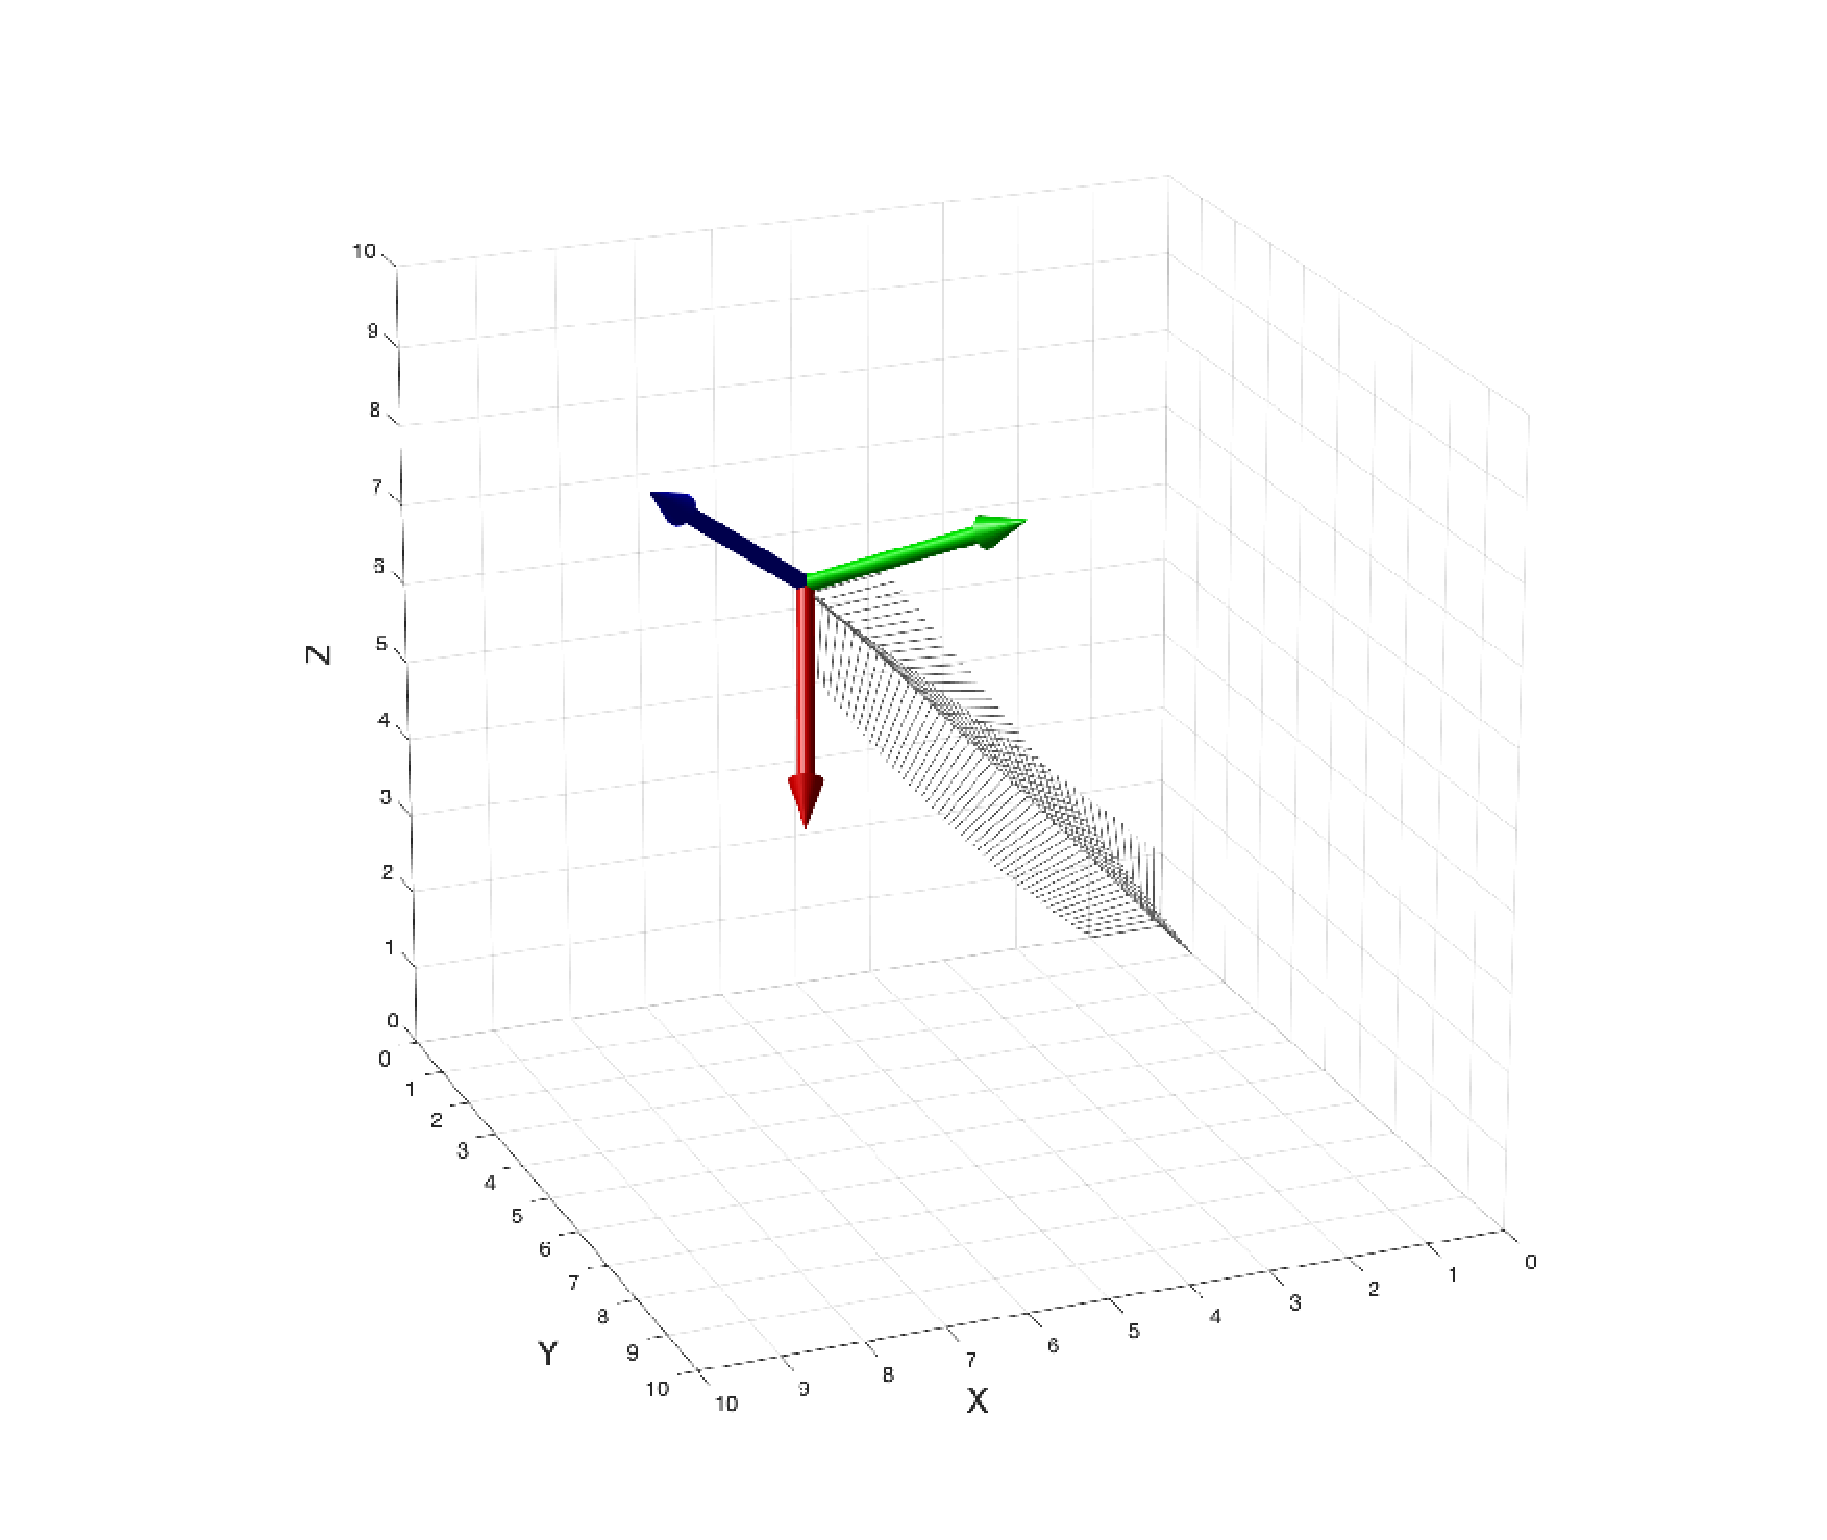
\includepdf{titlepage}
\fontsize{75}{80}\selectfont
\textbf{Spatial Math}\\[5pt]
\fontsize{45}{50}\selectfont
\textbf{Toolbox} for MATLAB\textsuperscript{\textregistered}\\[12pt]
Release \release

\vspace*{18cm}
\hfill\textbf{Peter Corke}\\[5pt]
\end{textblock}
\thispagestyle{empty}
\newpage
%%%%%%%%%%%%%%%%% INSIDE FRONT COVER
\typeout{**Inside front cover}
\vspace*{\fill}
\begin{tabular}{ll}
Release & \release \\
Release date & \reldate \\[20pt]
Licence & MIT \\
Toolbox home page &  \url{https://github.com/petercorke/spatial-math} \\
Discussion group & \url{https://tiny.cc/rvcforum}
\end{tabular}
\vspace*{\fill}
\hrule
Copyright \textcopyright \rtbyear\ Peter Corke\\
peter.i.corke$@$gmail.com\\
\url{http://www.petercorke.com}
\vspace*{\fill}
\setlength{\fboxsep}{10pt}%
\typeout{done}

%%%%%%%%%%%%%%%% CONTENT
\pagestyle{headings}        % Gives page headings at top of page
\lfoot{Spatial Math Toolbox \release\ for \Mlab\textsuperscript{\textregistered} }
\rfoot{Copyright \copyright Peter Corke \rtbyear}

\setcounter{section}{0}
\addcontentsline{toc}{section}{Preface}
\chapter*{Preface}
\typeout{**Preface front cover}
\pagestyle{fancyplain}
\begin{wrapfigure}{l}{4cm}
\vspace{-2ex}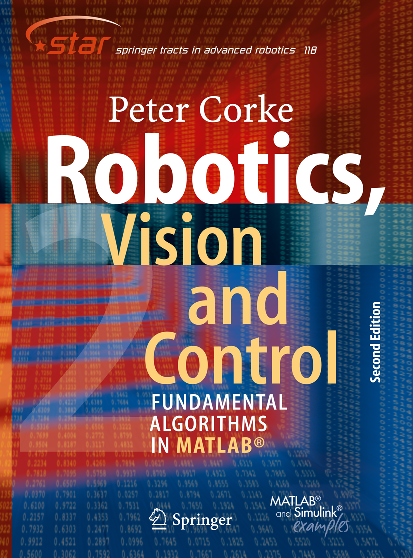
\includegraphics[width=3.5cm]{figs/frontcover.pdf}
\end{wrapfigure}
This is the first release of the Spatial Math Toolbox which has been refactored from the Robotics Toolbox for MATLAB.
The latter represents over twenty five years of continuous
development and a substantial level of maturity -- a significant part of that code base was concerned with representing position, orientation
and pose in 2D and 3D as well as lines in 3D using Pl\"{u}cker coordinates.

This \Mlab\textsuperscript{\textregistered} Toolbox has a rich collection of functions for manipulating and converting between datatypes such as vectors, rotation matrices, unit-quaternions, quaternions, homogeneous transformations and twists which are necessary to represent  position and orientation in 2- and 3-dimensions.
These are useful in the study of robotics and computer vision, but also for other fields of engineering and physics.

The Toolbox makes strong use of classes to represent many of the mathematical objects and also 
includes Simulink\textsuperscript{\textregistered} blocks for some conversions.
The code is written in a straightforward manner which allows
for easy understanding, perhaps at the expense of computational efficiency.
If you feel strongly about computational efficiency then you can always
rewrite the function to be more efficient,
compile the M-file using the \Mlab\   compiler, or
create a MEX version.

The bulk of this manual is auto-generated from the comments in the \Mlab\ code itself.
For elaboration on the underlying principles, extensive illustrations and worked examples please consult
 ``\textit{Robotics, Vision \& Control}''  which provides a detailed discussion (720 pages, nearly 500 figures and over 1000 code examples) of how to use the Toolbox functions to solve many types of problems in robotics.
This version corresponds to the \textbf{second edition} of the book ``\textit{Robotics, Vision \& Control}'' published in June 2017 -- aka RVC2.

%\cleardoublepage
%\chapter*{Functions by category}
%\addcontentsline{toc}{section}{Functions by category}
%\begin{multicols}{2}
%\IfFileExists{funcidx_body.tex}{\input{funcidx_body.tex}}{} 
%\end{multicols}

\cleardoublepage
\tableofcontents

\newpage
\chapter{Introduction}

As already mentioned this code has been refactored from the Robotics Toolbox for MATLAB.  As that Toolbox evolved there has been
increasing adoption of classes, even for objects like rotation matrices and homogeneous transformation matrices which can be
represented easily using native MATLAB matrices.  The motivations for this are:
\begin{enumerate}
\item Classes ensure type safety.  For example a 3x3 matrix could be an SO(3) rotation matrix or an SE(2) homogeneous transformation, or the transpose of an SE(3) homogeneous transformation is invalid.
Overloaded class operators ensure that only valid operations can be performed.
\item The classes support more descriptive constructors with names like \texttt{SO3.eul} which constructs an SO(3) object from Euler angles.
\item A sequence, or trajectory, using native matrices, has to represented by a 3-dimensional matrix, eg. $4\times 4 \times N$.  Using objects we can represent this instead using a 1-dimensional vector of objects.
\end{enumerate}
 
In RTB10 a set of classes have been introduced to represent orientation and pose in 2D and 3D: \texttt{SO2}, \texttt{SE2}, \texttt{SO3}, \texttt{SE3}, \texttt{Twist} and \texttt{UnitQuaternion}.  These classes are fairly polymorphic, that is, they share many methods and operators\footnote{For example, you could substitute objects of class \texttt{SO3} and \texttt{UnitQuaternion} with minimal code change.}.  All have a number of static methods that serve as constructors from particular representations.  A trajectory is represented by a vector of these objects which makes code easier to read and
understand.  Overloaded operators are used so the classes behave in a similar way to native matrices\footnote{The capability is extended so that we can element-wise multiple two vectors of transforms, multiply one transform over a vector of transforms or a set of points.}.
The relationship between the classical Toolbox functions and the new classes are shown in Fig \ref{fig:newfunctions}.

You can continue to use the classical functions.  The new classes have methods with the names of classical functions to provide similar functionality.  For instance
\begin{Code}
>> T = transl(1,2,3);  % create a 4x4 matrix
>> trprint(T)  % invoke the function trprint
>> T = SE3(1,2,3);  % create an SE3 object
>> trprint(T)  % invoke the method trprint
>> T.T   % the equivalent 4x4 matrix
>> double(T) % the equivalent 4x4 matrix
\end{Code}

\begin{Code}
>> T = SE3(1,2,3);  % create a pure translation SE3 object
>> T2 = T*T;  % the result is an SE3 object
>> T3 = trinterp(T, T2,, 5); % create a vector of five SE3 objects between T and T2
>> T3(1)  % the first element of the vector
>> T3*T  % each element of T3 multiplies T, giving a vector of five SE3 objects
\end{Code}

\begin{figure}[p]
\centering
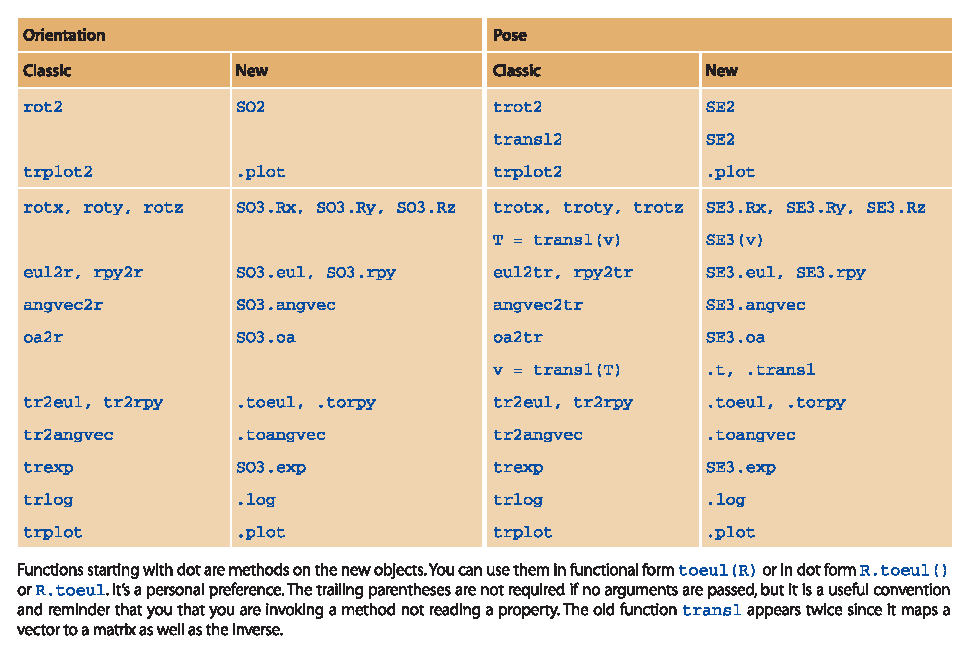
\includegraphics[width=\textwidth]{figs/CT-02-03.eps}
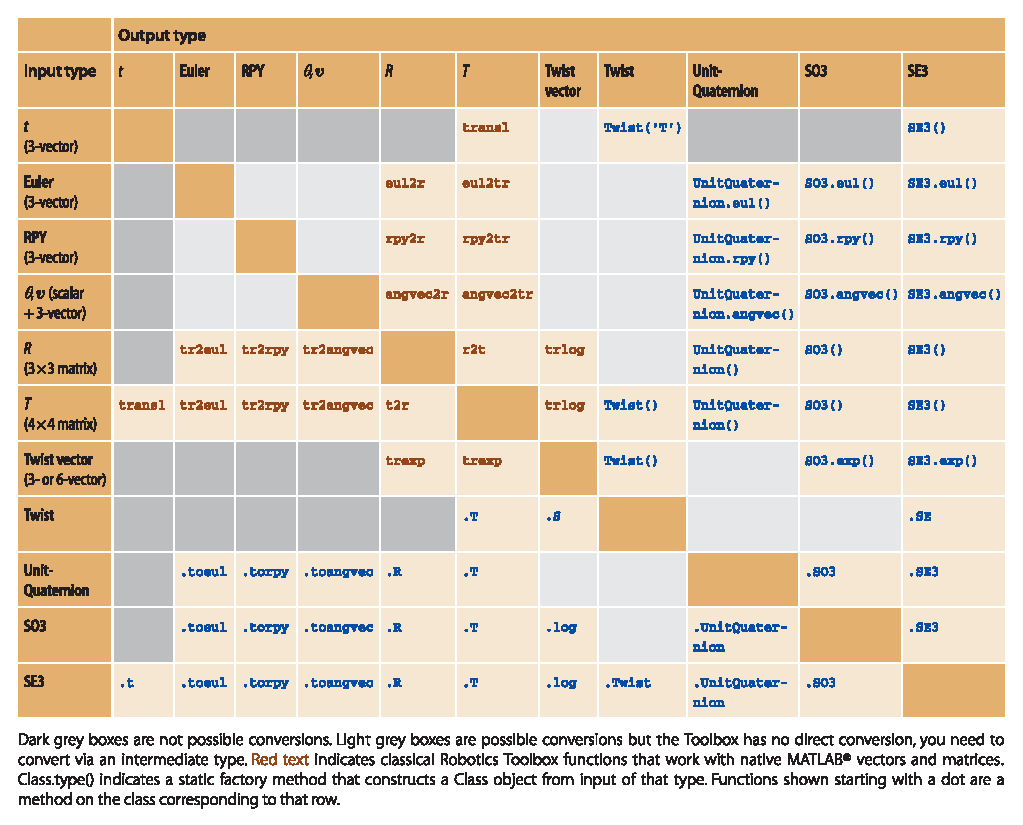
\includegraphics[width=\textwidth]{figs/CT-02-02.eps}
\caption{(top) new and classic methods for representing orientation and pose, (bottom) functions and methods to convert
between representations.  Reproduced from ``\textit{Robotics, Vision \& Control, second edition, 2017}''}\label{fig:newfunctions}
\end{figure}



Options to RTB functions can now be strings\footnote{Introduced from MATLAB 2016b.} or character arrays, ie. \texttt{rotx(45, 'deg')} or \texttt{rotx(45, "deg")}.  

\section{Installing the Toolbox}

\subsection{Automatically from GitHub}
From MATLAB Desktop or Online use the AddOn Manager on the Home tab, and search for "spatial math" and click on the Spatial Math Toolbox.
It will be installed into the folder \texttt{MATLAB/Add-Ons/Collections/Spatial Math Toolbox/petercorke-spatial-math-xxxx} in your default MATLAB
documents folder\footnote{\texttt{xxxx} is part of git's hash and represents the version number.}.

This also works from MATLAB Online in which case it will be stored in  \texttt{/MATLAB Add-Ons/Collections/Spatial Math Toolbox/petercorke-spatial-math-xxxx}.

The Toolbox will be automatically added to the end of your path.  If you have the Phase Array Toolbox also installed then note that some of the Spatial Math functions will be shadowed.  To check for this run
\begin{Code}
>> which rotx
\end{Code}
If this indicates a path not as shown above then  either:
\begin{enumerate}
\item use \texttt{pathtool} to move Phase Array Toolbox to the end of the path
\item remove the Phase Array Toolbox, if you don't need it, using the AddOn Manager. 
\end{enumerate}

\subsection{Manually from GitHub}
Clone the repository to your own computer
\begin{Code}
>> git clone https://github.com/petercorke/spatial-math
\end{Code}
and ensure that the folder \texttt{spatial-math} is added to your MATLAB path.


\subsection{Notes on implementation and versions}
The Simulink blocks are implemented in Simulink itself with calls to MATLAB code, or as Level-1 S-functions (a proscribed coding format which MATLAB functions
to  interface with the Simulink simulation engine).

Simulink allows signals to have matrix values but not (yet) object values.  Transformations must be represented as matrices, as per the classic functions, not classes.
Very old versions of Simulink (prior to version 4) could only handle scalar signals which limited its usefulness for robotics.

\subsection{Documentation}
This document {\tt spatialmath.pdf} is a comprehensive manual that describes all functions in the Toolbox.
It is auto-generated from the comments in the \Mlab\ code and is fully hyperlinked:
to external web sites, the table of content to functions, and the ``See also'' functions
to each other.

%The same documentation is available online in
%alphabetical order at \url{http://www.petercorke.com/RTB/r10/html/index_alpha.html}
%or by category at \url{http://www.petercorke.com/RTB/r10/html/index.html}.
%Documentation is also available via the \Mlab\ help browser,  under supplemental software, as ``Robotics
%Toolbox".


\section{Compatible MATLAB versions}
The Toolbox has been tested under R2018b and R2019aPRE.  Compatibility problems are increasingly likely the older your version of \Mlab\ is.

\section{Use in research}
If the Toolbox helps you in your endeavours then I'd appreciate you citing the Toolbox when you publish.
The details are:
\begin{verbatim}
@book{Corke17a,
    Author = {Peter I. Corke},
    Note = {ISBN 978-3-319-54413-7},
    Edition = {Second},
    Publisher = {Springer},
    Title = {Robotics, Vision \& Control: Fundamental Algorithms in {MATLAB}},
    Year = {2017}}
\end{verbatim}
or
\begin{quote}
P.I. Corke, Robotics, Vision \& Control: Fundamental Algorithms in MATLAB. Second edition. Springer, 2017. ISBN 978-3-319-54413-7.
\end{quote}
which is also given in electronic form in the CITATION file.


\subsection{Octave}
GNU Octave (www.octave.org) is an impressive piece of free software that implements a language that is close to, but not the same as, \Mlab. The Toolboxes currently do not work well with Octave, though as time goes by compatibility improves.  
Many Toolbox functions work just fine under Octave, but most classes do not.

For uptodate information about running the Toolbox with Octave check out the page \url{http://petercorke.com/wordpress/toolboxes/other-languages}.



\section{Support}
There is no support!  This software is made freely available in the hope that you find it useful in solving whatever problems
you have to hand.
I am happy to correspond with people who have found genuine
bugs or deficiencies but my response time can be long and I can't guarantee that I respond to your email.

\textbf{I can guarantee that I will not respond to any requests for help with assignments or homework, no matter
how urgent or important they might be to you.  That's what your teachers, tutors, lecturers and professors are paid to do.}

You might instead like to communicate with other users via 
the Google Group called ``Robotics and Machine Vision Toolbox'' 
\begin{quote}
\url{http://tiny.cc/rvcforum}
\end{quote}
which is a forum for discussion.
You need to signup in order to post, and the signup process is moderated by me so allow a few
days for this to happen.  I need you to write a few words about why you want to join the list
so I can distinguish you from a spammer or a web-bot.



\section{Contributing to the Toolboxes}
I am very happy to accept contributions for inclusion in future versions of the
toolbox.  You will, of course, be suitably acknowledged.

\renewcommand{\section}{\funcsection}
%\setcounter{secnumdepth}{-1}
%\settocdepth{section}
\newpage
\chapter{Functions and classes}
\typeout{**Before include}
\IfFileExists{all.tex}{\input{all}}{} 
\typeout{**After include}

\bibliographystyle{ieeetr}
\bibliography{strings,robot,control,dynamics,kinematics,force,grind,publist,software}
\end{document}
